\documentclass{article}
\usepackage[paperwidth=188mm,paperheight=160mm,margin=4mm]{geometry}
\usepackage{graphicx}
\usepackage{tikz}
\usetikzlibrary{arrows.meta,positioning,fit,backgrounds,calc}
\pagestyle{empty}

\begin{document}
\noindent\resizebox{\textwidth}{!}{%
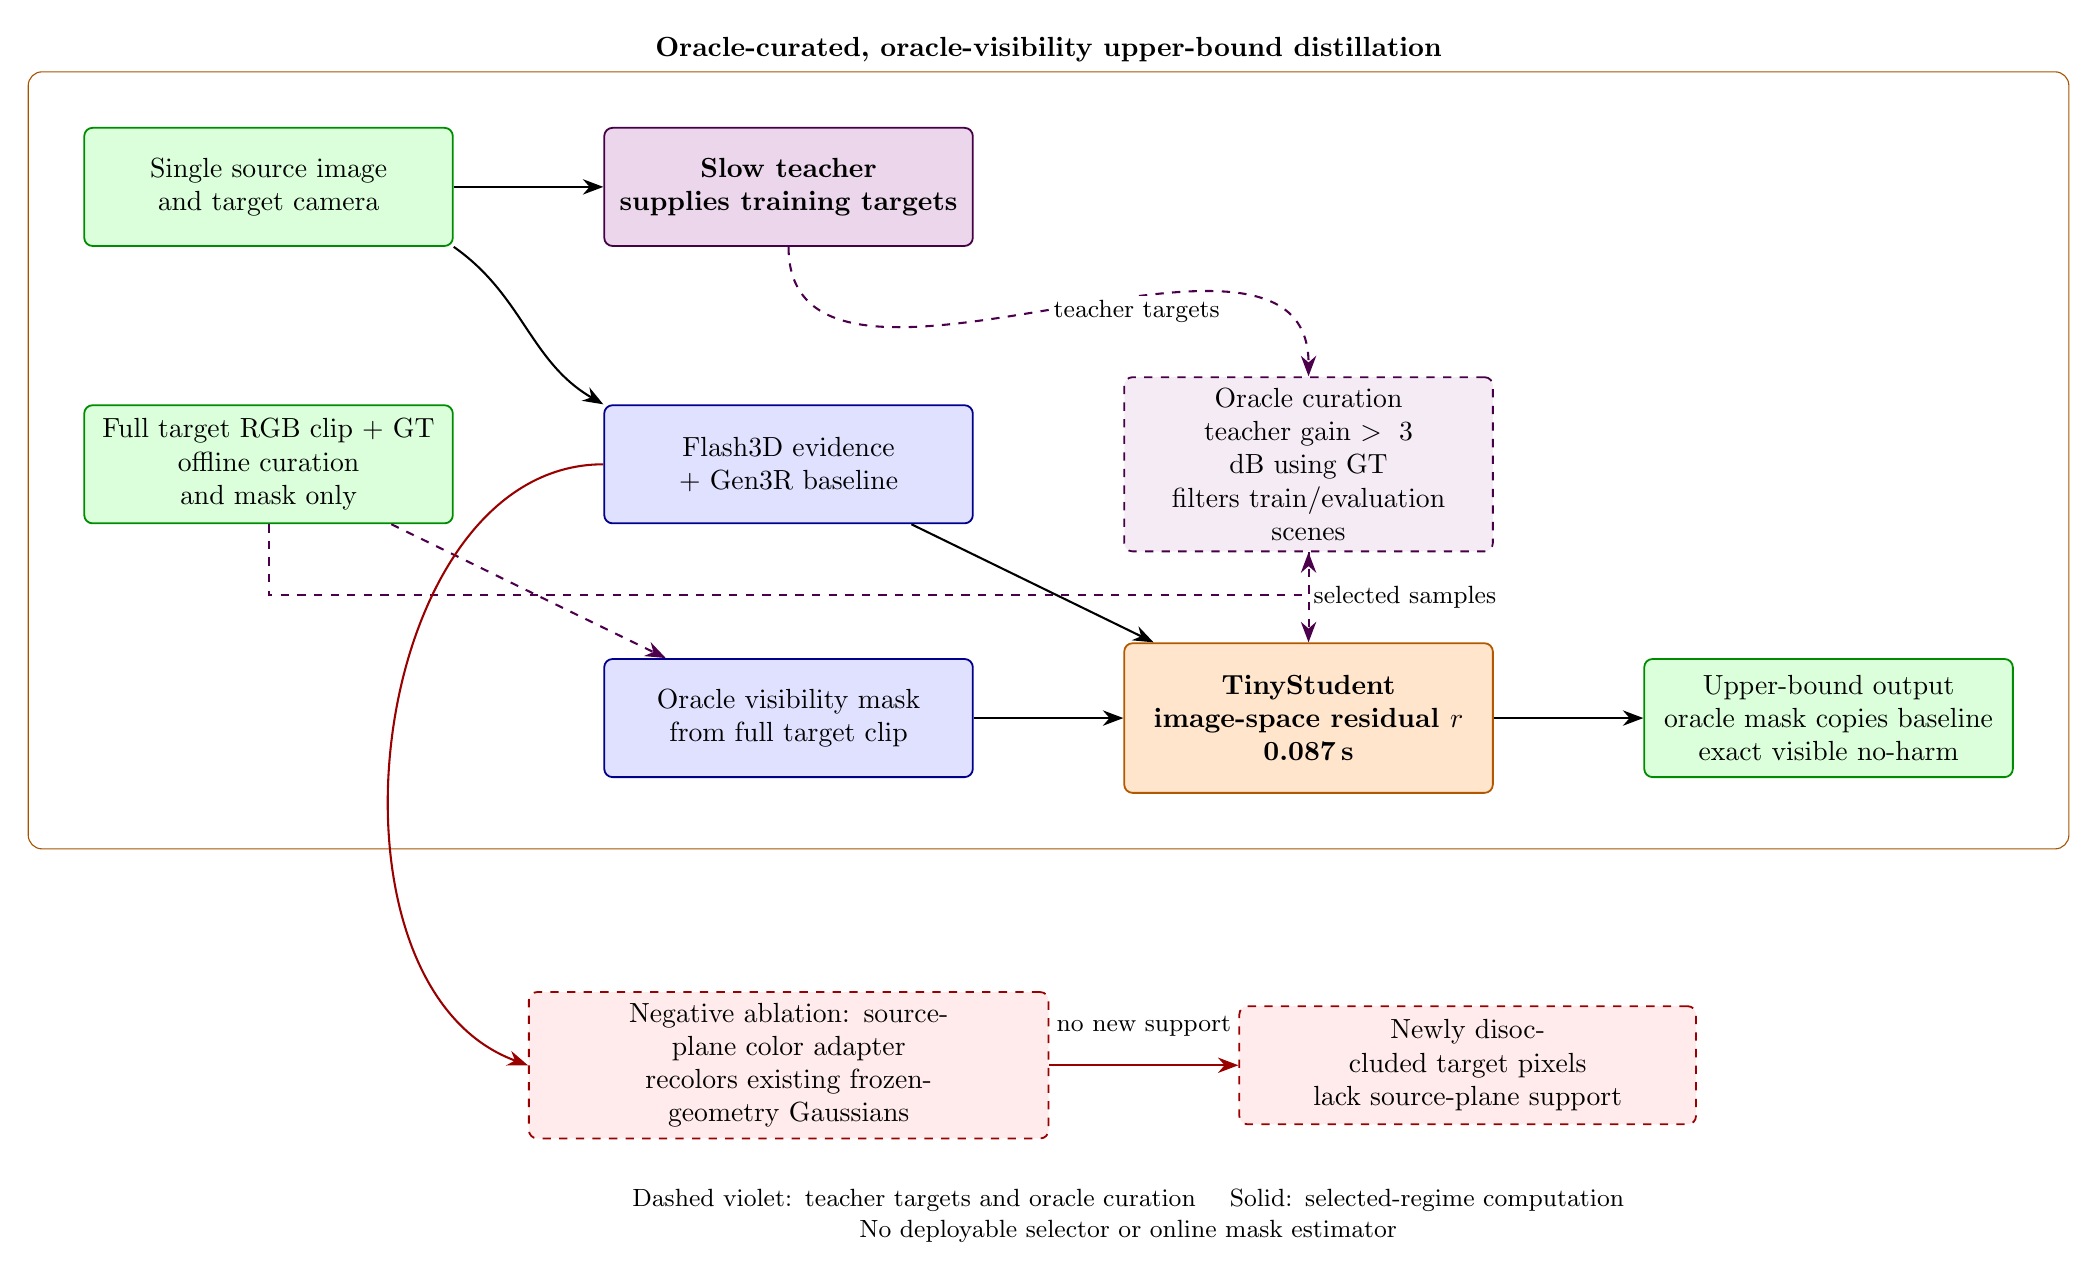
\begin{tikzpicture}[
  font=\normalsize,
  >={Stealth[length=2.6mm]},
  box/.style={rounded corners=3pt,draw,align=center,minimum height=15mm,text width=44mm,inner sep=4pt,line width=0.65pt},
  input/.style={box,fill=green!14,draw=green!55!black},
  teacher/.style={box,fill=violet!16,draw=violet!55!black,font=\normalsize\bfseries},
  selection/.style={box,fill=violet!8,draw=violet!55!black,dashed},
  student/.style={box,fill=orange!20,draw=orange!70!black,font=\normalsize\bfseries},
  evidence/.style={box,fill=blue!12,draw=blue!55!black},
  unsupported/.style={box,fill=red!8,draw=red!60!black,dashed},
  arr/.style={->,line width=0.75pt},
  train/.style={->,line width=0.75pt,dashed,draw=violet!60!black},
  edge/.style={font=\small,fill=white,inner sep=1.5pt},
]

\node[input] (inputs) {Single source image\\and target camera};
\node[teacher,right=19mm of inputs] (teacher) {Slow teacher\\supplies training targets};
\node[input,below=20mm of inputs] (oracledata) {Full target RGB clip + GT\\offline curation and mask only};
\node[evidence,right=19mm of oracledata] (evidence) {Flash3D evidence\\+ Gen3R baseline};
\node[selection,right=19mm of evidence] (selection) {Oracle curation\\teacher gain $>3$ dB using GT\\filters train/evaluation scenes};
\node[evidence,below=17mm of evidence] (mask) {Oracle visibility mask\\from full target clip};
\node[student,right=19mm of mask,minimum height=19mm] (student) {TinyStudent\\image-space residual $r$\\0.087\,s};
\node[input,right=19mm of student] (output) {Upper-bound output\\oracle mask copies baseline\\exact visible no-harm};

\draw[arr] (inputs) -- (teacher);
\draw[arr] (inputs.south east) to[out=-35,in=150] (evidence.north west);
\draw[train] (oracledata) -- (mask);
\draw[train] (teacher.south) to[out=-90,in=90] node[edge,right]{teacher targets} (selection.north);
\draw[train] (oracledata.south) -- ++(0,-9mm) -| (selection.south);
\draw[train] (selection.south) -- node[edge,right]{selected samples} (student.north);
\draw[arr] (evidence) -- (student);
\draw[arr] (mask) -- (student);
\draw[arr] (student) -- (output);

\begin{scope}[on background layer]
  \node[draw=orange!65!black,rounded corners=5pt,fit=(inputs)(teacher)(oracledata)(selection)(evidence)(mask)(student)(output),inner sep=7mm,label={[font=\bfseries]above:Oracle-curated, oracle-visibility upper-bound distillation}] (pipeline) {};
\end{scope}

\node[unsupported,below=18mm of pipeline.south,xshift=-33mm,minimum width=66mm] (adapter) {Negative ablation: source-plane color adapter\\recolors existing frozen-geometry Gaussians};
\node[unsupported,right=24mm of adapter,minimum width=58mm] (hole) {Newly disoccluded target pixels\\lack source-plane support};
\draw[arr,draw=red!60!black] (adapter) -- node[edge,above=3mm]{no new support} (hole);
\draw[arr,draw=red!60!black] (evidence.west) to[out=180,in=160] (adapter.west);
\node[font=\small,anchor=north,align=center,text width=170mm] at ($(adapter.south)!0.5!(hole.south)+(0,-6mm)$)
  {Dashed violet: teacher targets and oracle curation \quad Solid: selected-regime computation\\No deployable selector or online mask estimator};

\end{tikzpicture}%
}
\end{document}
